Apache Derby is an open-source Java \ac{rdbms}, that has a very small footprint (about 2.6MB of disk-space for the base engine and embedded \ac{jdbc} driver \cite{derbySite}). The on-disk database format used in Derby is portable and platform-independent, meaning that the database can be moved from machine to machine with no need to modify the data, and that the database will work with any derby configuration \cite{derby10}. 

A Derby database exists within a system (Fig. \ref{fig:derbystruct}), composed by a single instance of the Derby database engine and the environment in which it runs. It consists of zero or more databases, a system-wide configuration and an error log, both contained in the system directory \cite{derbyDev10}.

\begin{figure}[htb]
  \begin{center}
    \leavevmode
    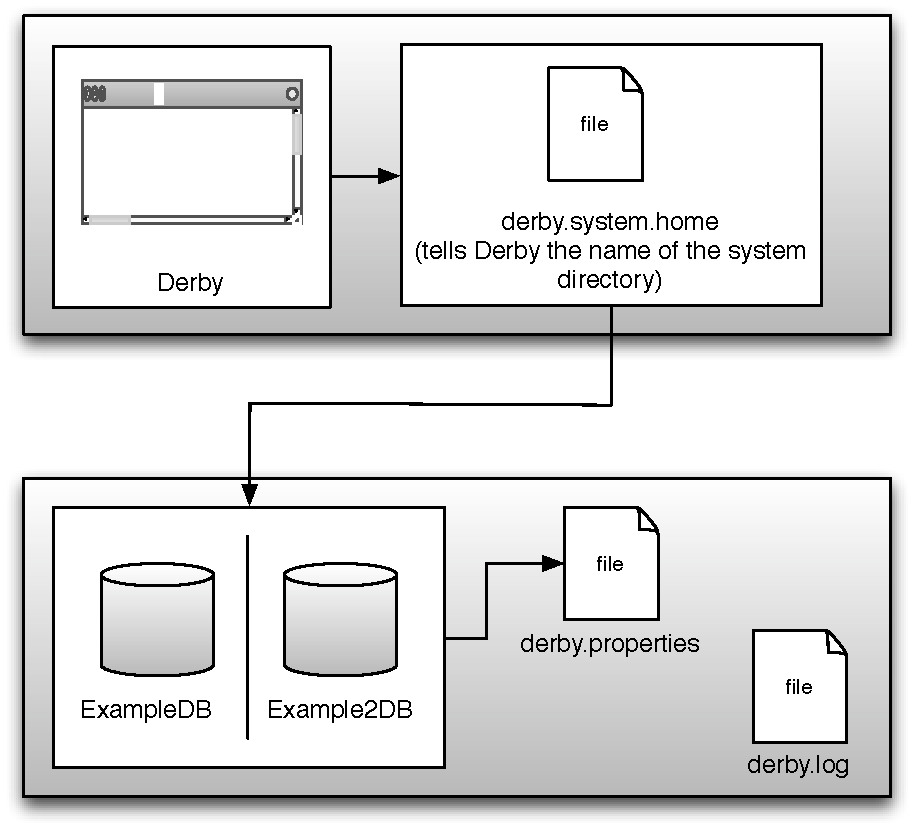
\includegraphics[width=0.5\textwidth]{images/derbystruct}
  \end{center}
  \caption{Derby System Structure}
  \label{fig:derbystruct}
\end{figure}

\section{Data Model}
Derby's data model is relational, implying that data can be accessed and modified using \ac{jdbc} and standard \ac{sql}. The system has, however, two very different basic deployment options (or frameworks), the simple embedded option and the Derby Network Server option \cite{derby10}. 

\begin{description}
	\item[Embedded] In this mode Derby is started by a single-user Java application, and runs in the same Java virtual machine (JVM). This makes Derby almost invisible to the user, since it is started and stopped by the application, requiring very little or no administration. This has the particularity that only a single application can access the database at any one time, and no network access occurs. 
	\item[Server (or Server-based)] In this mode Derby is started by an application that provides multi-user connectivity to Derby databases across a network. The system runs in the JVM that hosts the server, and other JVM's connect to it to access the database.
\end{description}	

\section{Querying}
Querying in Derby is done, as previously mentioned, with the usage of \ac{sql}, more precisely features from \ac{sql}-92 \cite{derbySQL}.

\ac{sql} scope includes data insert, query, update and delete, schema creation and modification, and data access control, and is the most widely used language for relational databases \cite{SQLintro}. \ac{sql} statements are executed by a database manager, who also has the function transforming the specification of a result table into a sequence of internal operations that optimize data retrieval. This transformation occurs in two phases: preparation and binding.

All executable \ac{sql} statements must be prepared before they can be executed, with the result of this preparation being the executable or operational form of the statement. The method of preparing an \ac{sql} statement and the persistence of its operational form distinguish static \ac{sql} from dynamic \ac{sql} \cite{SQLibm}.

\section{Consistency}
Derby databases provide ACID guarantees, according to the ACID test \cite{derbydevIBM}. This means that operations with the database can be grouped together and treated as a single unit (atomicity), it makes sure that either all the operations in this single unit (\emph{transaction}) are performed, or none is (consistency), also, independent sets of database transactions are performed so that they don't conflict with each other (isolation) and it also guarantees that the database is safe against unexpected terminations (durability).

\section{Patching Derby}

The idea of patching Derby so that the data is stored in a different way is not entirely new and was firstly introduced by Knut Magne Solem\cite{derbyPatch}. In his approach all the tables whose name began with \emph{MEM} were stored in memory, following the same strategy, our approach stores in Cassandra all the tables whose name starts with \emph{TUPLE}.

This implies re-writing all the classes and methods from the access part of the Derby engine, that uses a BTree by default and therefore are in the namesake package. As this implementation uses a Tuple Store, the name of the package was also tuplestore.

When rewriting this classes some optimizations were made, such as the reutilization of connections since Derby creates one physical connection to the underlying database for each transaction, which could mean a reasonable overhead when a new one was created due to the cost of establishing the connection. To circumvent this, a pool of connections is created and if there is one free it is used, otherwise a new connection is opened, preventing some of the overhead. 

\subsection{Records}

\subsection{Indexing}
Indexing is a way of sorting a number of records on multiple fields. Creating an index on a field in a table creates another data structure with the field value, and a pointer to the primary record. 

The downside to indexing is that these indexes require additional space on the disk and processing time when inserting new data.

\subsubsection{Derby Indexes}
Parallel to the actual record handling classes, there are the ones responsible for the indexes, which can be of one of three types:

\begin{description}
	\item[Primary] Refers to primary keys. There can only be one per table and it must unambiguously match one, and only one, record.
	\item[Unique] Resemble ordinary (secondary) indexes, except they prevent duplicates from being added.
	\item[Secondary] Secondary or Ordinary indexes serve the same purposes as primary indexes, but on different values than the primary key.
\end{description} 

The creation of an index in the patched version of Derby depends on its type. 

In the case where it is a primary index, Derby is informed about it (through a flag), but no actual index is created, since the record already contains that information and is indexed for it.

On the rest of the cases, an index is created according to the model defined in chapter \todo{capitulo do modelo de dados do cassandra}.

When fetching information that is indexed, Derby first estimates the cost of fetching using the index or not, based on the number and size of the rows, and acts accordingly.

\begin{figure}[h]
  \centering    
  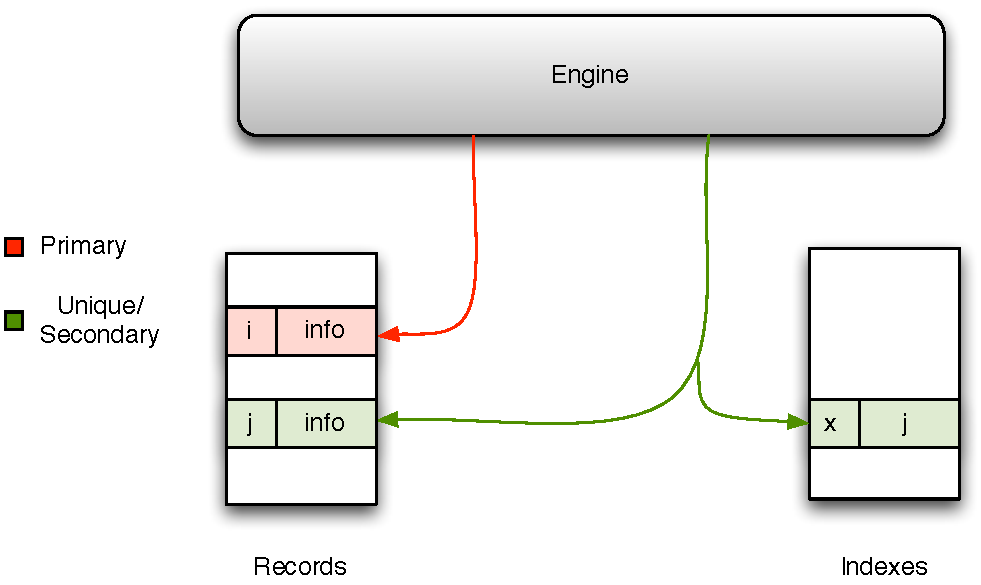
\includegraphics[width=0.9\textwidth]{images/derbyindexes}
  \caption{Derby Indexes}
  \label{fig:derbyindexes}
\end{figure}


\subsection{Scans}

\todo[inline]{Explicar como é feito uma range query no Derby}  

When performing a scan that involves fetching a row through an index, Derby gets the row for that index from which it extracts the location of the actual record and then does a second fetch, this time to the location pointed by the index.

This is fine for unique and secondary indexes, but as explained in the previous section, in the case of primary indexes there is no need for the creation of a specific row for the index, thus making this two fetches mechanism redundant. Since this redundancy meant an unnecessary access to the database, which could incur in a large overhead, this matter had to be addressed. 

The way this was solved was by storing in memory the whole row fetched in first place (through the index) and passing it on alongside with the actual record location. This allows for the controller of the fetch to use the information in memory, when it is available.   








